%%This is a very basic article template.
%%There is just one section and two subsections.
\documentclass{article}
\usepackage{amsmath}
\usepackage{float}
\usepackage{graphicx}

\begin{document}
\newcommand{\bx}{\mathbf{x}}
\newcommand{\ddq}{\frac{\partial}{\partial \epsilon_t}}
\newcommand{\dxdq}{\frac{\partial \bx}{\partial \epsilon_t}}
\newcommand{\argmin}{\operatornamewithlimits{argmin}}
\newcommand{\argmax}{\operatornamewithlimits{argmax}}
 \newcommand{\Prob}{\text{P}}
 \newcommand{\Z}{\textbf{Z}}
\section{Dense 3D Reconstruction using Robot Hand-Mounted Cameras}

This is a general sketch of an idea for reconstructing a dense 3D scene using a
hand-mounted depth camera.

\subsection{Problem}

Consider a robot that has a configuration space $C \subseteq \mathbf{R}^N$.
Mounted on one of the links of the robot is a depth sensor. The task is, given a
sequence of noisy configurations at each time step $\{q_1, q_2, \ldots,
q_T\} \in C$, and a sequence of noisy sensor readings (point clouds) captured
simultaneously $\Z = \{Z_1, Z_2, \ldots, Z_T\}$, where $Z_i = \{\bx_1, \ldots,
\bx_N\} \subseteq \mathbf{R}^3$,  simultaneously reconstruct the true dense 3D
geometry of the scene and estimate the true configuration of the robot at each time step.

\subsection{Configuration Noise Model} 

The robot's configuration at time step $t$ is given by joint encoder readings
$q_t$, which is a random value drawn from the distribution:

$$q_t = q_t^{\text{true}} + \epsilon_t$$

\noindent Where $q_t^{\text{true}}$ are the true joint angles of the robot,
and $\epsilon_t$ is a random offset drawn from some unknown random distribution
$Q$.

$$ \epsilon_t \sim \text{Q}(q_t^{\text{true}}) $$

In practice, $\text{Q}$ is highly nonlinear, and depends on the dynamics of the
system (for example, the direction of gravity, or other factors that depend
on the robot's joint angles). Therefore, finding an \emph{a. priori}
represention of $\text{Q}$ may be infeasible. The task is to compute $\epsilon^*_t$, which is an estimate of the
current noisy offset.

\subsection{General Approach} 

We want to find the maximum likelihood estimate of $\epsilon_t$ given the sensor readings at time $t$:

\begin{align}
\epsilon^*_t  &= \argmax_{\epsilon_t} \Prob\left(\epsilon_t | \Z_t\right)  \\
							&= \argmax_{\epsilon_t} \frac{\Prob\left(\Z_t |	\epsilon_t\right)\Prob\left(\epsilon_t\right)}{\Prob\left(\Z_t\right)} \\
							&= \argmax_{\epsilon_t} \frac{ \Prob\left(\epsilon_t\right)\prod_{\bx_i \in \Z_t}{\Prob\left(\bx_i | \epsilon_t\right)}}{\Prob\left(\Z_t\right)}  \\
							&= \argmax_{\epsilon_t} \log \frac{ \Prob\left(\epsilon_t\right)\prod_{\bx_i \in \Z_t}{\Prob\left(\bx_i |	\epsilon_t\right)}}{\Prob\left(\Z_t\right)}  \\
						    &= \argmax_{\epsilon_t}  \left[\log\Prob\left(\epsilon_t\right) + \sum_{\bx_i \in \Z_t}{\log \Prob\left(\bx_i |	\epsilon_t\right)} - \log \Prob\left(\Z_t\right)\right] \\
						    &= \argmax_{\epsilon_t}  \left[\log\Prob\left(\epsilon_t\right) + \sum_{\bx_i \in \Z_t}{\log \Prob\left(\bx_i |	\epsilon_t\right)}\right]
\end{align}

The term $\Prob\left(\epsilon_t\right) = \text{Q}(q_t^{\text{true}})$ is the prior on $\epsilon_t$. The individual terms $\Prob\left(\bx_i | \epsilon_t\right)$ are the posterior probabilities of each sensor reading given a particular configuration
offset $\epsilon_t$. Calculating this term will require a defintion of the world, and the properties of the sensor.

\subsection{World Representation}

We will represent the world as a truncated signed distance function (TSDF). It
is defined as $D(\bx) : \mathbf{R}^3 \to \mathbf{R}$, and represents the
(signed) distance to the nearest obstacle in meters, up to a truncation distance $\tau$.

The gradient of the distance field $\nabla D : \mathbf{R}^3 \to \mathbf{R}^3$,
is clearly defined and easy to compute.

\subsection{Forward Kinematics}

Assume we have a forward kinematics function of the robot $\text{F(q, x)} : \mathbf{R}^N \times \mathbf{R}^3 \to \mathbf{R}^3$ which maps points in the frame of the sensor to the world.

\subsection{Sensor Noise Model}

\begin{figure}
	\centering
	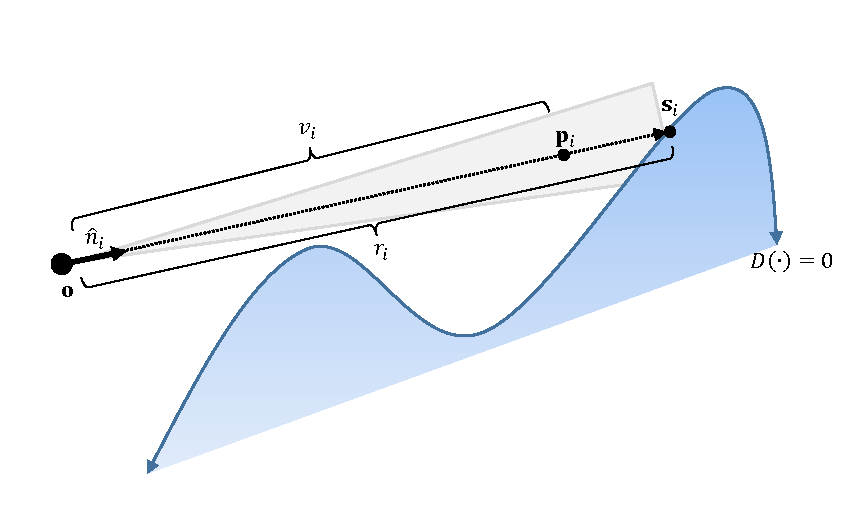
\includegraphics[width=1.0\textwidth]{img/raycone.pdf}
	\caption{The sensor has origin $\mathbf{o}$, a cone is cast out of the sensor with direction $\hat{n}_i$. The ray through the center of the cone intersects the world at point $\mathbf{s}_i$, and the point implied by the range reading is given by
	$\mathbf{p}_i$. The expected range is $r_i$, and the observed range is $v_i$.} 
	\label{fig:ray_cone} 
\end{figure}

Consider the typical ray-cone sensor model for lasers and other depth sensors. In this model, each point $\bx_i$ actually represents a \textit{cone} of rays emenating from the sensor's origin. If the cone hits any surface in the scene, the depth
sensor returns a noisy reading of the range from the sensor to that point. If multiple surfaces intersect the cone, the range reading returned randomly flips between the ranges to each surface with a distribution dependant on the amount of cone area
each intersected surface sweeps out. This sensor model makes $\Prob\left(\bx_i | \epsilon_t\right)$ quite complicated. 

\subsubsection{Ray Approximation}
 We can signficiantly simplify the problem by modeling the sensor reading as a single \textit{ray} passing through the center of the cone. The origin of the ray is given by $ \mathbf{o} = \text{F}(q_t +
\epsilon_t, \mathbf{0})$, and the endpoint of the ray is given by $\mathbf{p}_i =\text{F}(q_t + \epsilon_t, \bx_i)$.  The ray can be paramaterized by arc-length (Fig. \ref{fig:ray_cone}):

\begin{equation}
R_i(\alpha) = \mathbf{o} + \alpha \hat{n_i}  
\end{equation}

\noindent where $\alpha \in [0, r_i]$ is a range along the ray, and $\hat{n_i}$ is the unit normal direction of the ray. The likelihood of the ray can then be modeled by considering all points along the ray as independent readings:

\begin{equation}
\Prob(\bx_i | \epsilon_t, D) = \prod_{\alpha \in [0, r_i]} \Prob\left(R_i(\alpha) | D\right) 
\end{equation}

\noindent (note that this assumes each point along the ray is conditionally independent given the distance field $D$).  The distribution $\Prob(R_i(\alpha))$ will differ depending on $\alpha$. Points along the ray very near the sensor are much more
likely to be unoccupied than points very near the endpoint of the ray. Rays passing through solid objects should have very low probability. Rays with endpoints in empty space should also be very improbable. But rays merely \textit{grazing} surfaces
without passing through them should be expected around the silhouettes of objects. 

TODO: what is $\Prob\left(R_i(\alpha) | D\right) $?

\subsubsection{Ray Endpoint Approximation} 
If instead assume that the ray intersects only one surface, we can find the probability that we got a particular sensor reading by considering just the endpoint of the ray:

\begin{equation}
\Prob\left( \bx_i | \epsilon_t \right) \approx \Prob \left(\mathbf{p}_i | D \right)
\end{equation}

\noindent a simple model of $\Prob \left(\mathbf{p}_i | D \right)$ is that the range reading returned by the sensor is corrupted by Guassian noise. If that's the case, we can determine the expected range reading given the known world model, and
compare it to the observed range reading given $\mathbf{p}_i$. Assuming the ray actually intersects a surface in the scene, the expected range is given by raycasting to the surface:

\begin{equation}
r_i = \left\|\mathbf{o_i} +  \argmin_{\alpha \in [0, \infty)} \left[D(\mathbf{o}_i + \alpha \hat{n_i})^2\right] \hat{n}_i\right\|
\end{equation}


Then, if the range reading $v_i =\| \mathbf{p}_i - \mathbf{o}_i\| $ is drawn from the normal distribution:

\begin{equation}
v_i \sim \mathcal{N}_{r_i, \sigma_i}(x)= \frac{1}{\sigma_i \sqrt{2 \pi}} \exp{\frac{-(r_i - x)^2}{2 \sigma_i^2}}
\end{equation}

\noindent where $r_i$ is the mean of the distribution, and $\sigma_i$ is its standard deviation, we can compute:

\begin{equation}
\Prob \left(\mathbf{p}_i | D \right) = \mathcal{N}_{r_i, \sigma_i}(v_i)
\end{equation} 

Using this approximation ignores the presence of multiple surfaces, and the cone structure of the sensor reading,  but it at least takes into account the aniostropic (direction-dependant) range noise of the sensor.

\subsubsection{Simple Point Approximation}

An even simpler approximation of the sensor model ignores both the aniostropy of the noise, and the cone/ray structure of the scene by doing the following: for all surface points in the scene visible to the sensor, a reading is emitted that is the
surface point corrupted by linear Gaussian noise.

More precisely, call the set of all surface points visible to the sensor at configuration $q_t$ $\mathbf{S}_t$.  For a particular point $\mathbf{s}_i \in \mathbf{S}_t$, we observe a sensor reading:

\begin{equation}
\bx_i = \text{F}^{-1}\left(q_t, \mathbf{s}_i +\mathbf{d}_i\right)
\end{equation}

\noindent where $\text{F}^{-1} : \mathbf{R}^N \times \mathbf{R}^3 \to \mathbf{R}^3$ takes a point in the world frame and transforms it into the sensor frame given a configuration of the robot,  and $\mathbf{d}_i \sim \mathcal{N}_{\mathbf{0},
\Sigma_D}$ is random linear 3 dimensional Guassian noise with a covariance of $\Sigma_D$.

This (very inaccurate) model of the sensor essentially just ``fuzzes out'' all points seen by the robot.  Using this model, we can derive the posterior:

\begin{equation}
\Prob \left(\mathbf{p}_i | D \right) = \mathcal{N}_{\mathbf{0}, \Sigma_D}\left(D(p_i) \right)
\end{equation} 

\noindent that is, the probability of a sensor reading is proportional to the observed distance at the end point.

\subsection{Optimization} 

We will iteratively build up the TSDF. $D_t$ is calculated by first estimating a
configuration of the robot $q^*_t = q_t + \epsilon^*_t$ which minimizes the
squared error between the sensor measurements $Z_t$ and the previous TSDF model
$D_{t - 1}$.  Then, the sensor measurements are projected back into the world
given $q^*_t$, and the usual TSDF update is applied.

\begin{figure}
	\centering
	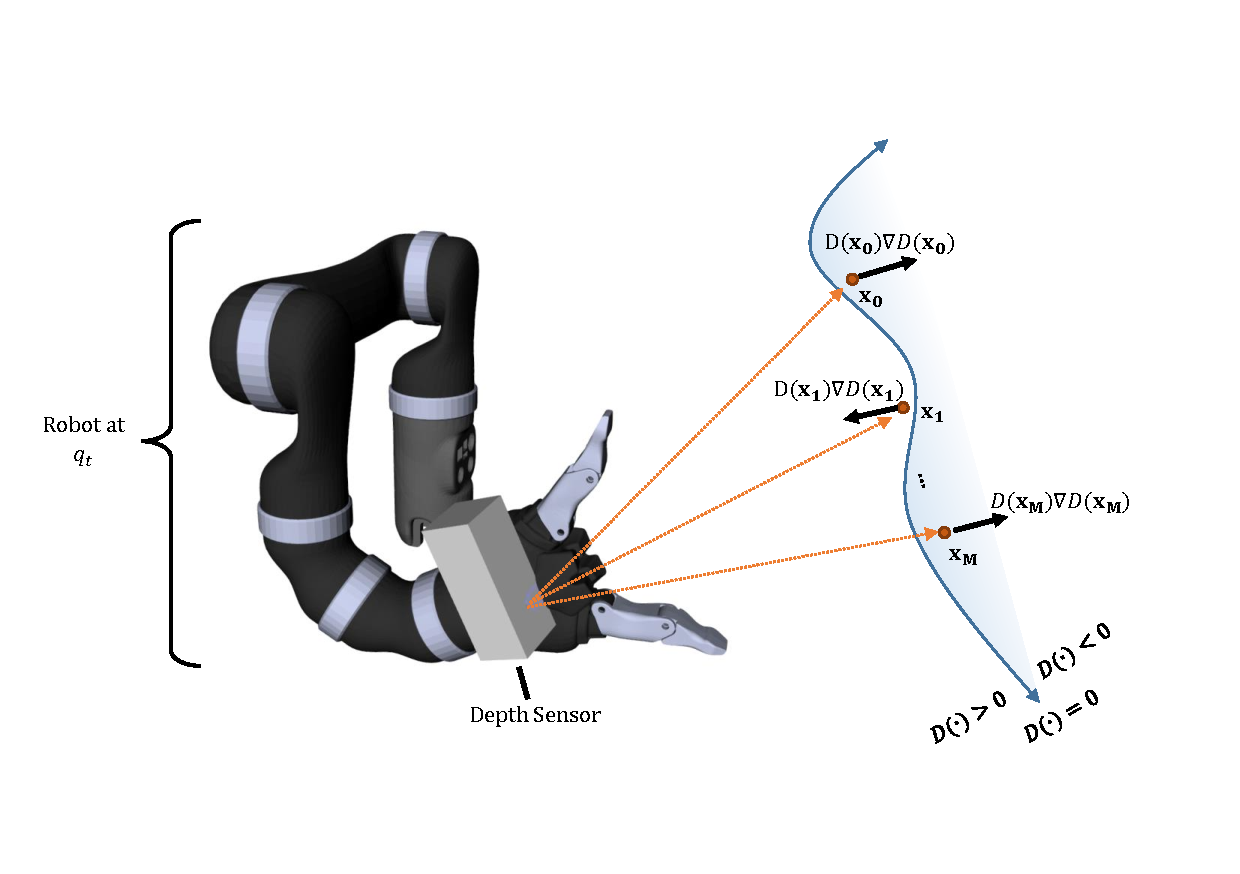
\includegraphics[width=1.0\textwidth]{img/robot_reconstruct.pdf}
	\caption{A diagram of the robot sensing a surface with a depth sensor. Rays
	from the depth sensor are shown as orange dotted lines. The point cloud
	$\{\bx_1, \ldots, \bx_M\}$ is used to determine the gradient of the distance
	field $\nabla D$ at each point.}
	\label{fig:robot} 
\end{figure}

\subsection{Computing $\epsilon^*_t$}

We can compute $\epsilon^*_t$ by performing \textbf{gradient descent} in the
configuration space of the robot.  Define the \textbf{forward kinematics
function} $F(q_t, Z_t) : \mathbf{R}^3 \to \mathbf{R}^3$, which merely
transforms the point cloud $Z_t$ into the world frame, given configuration $q_t
\in C$. Call

$$ F_t = F(q_t + \epsilon_t, z_t) $$

Then, the objective function $h(\epsilon_t, D_{t-1}) : C \to \mathbf{R}$ is
given by the sum squared distances of all of the projected points in $F_t$:

$$ h(\epsilon_t, D_{t-1}) = \sum_{x \in F_t}\left(D_{t-1}(x)\right) ^2 $$

Minimizing this objective function also maximizes the likelihood of the simple point approximation of the sensor model. (TODO: prove this).

\subsubsection{Computing the Gradient}

Now, we want to find the partial differential of $h$ with respect to
$\epsilon_t$:


\begin{align} 
\frac{\partial{h}}{\partial{\epsilon_t}} &= \ddq  \sum_{\bx \in F_t}\left(D_{t-1}(\bx)\right) ^2 \\
 &= \sum_{\bx \in F_t} \ddq \left(D_{t-1}(\bx)\right) ^2 \\ 
 &= 2\sum_{\bx \in F_t} D_{t-1}(\bx) \dxdq \nabla D_{t-1}(\bx)
\end{align} 

And, since $\dxdq$ is the change in $\bx$, a projected sensor point, with
respect to $\epsilon_t$, the configuration of the robot at time $t$, we have (with some
handwaving):

$$ \dxdq = J_\bx \in \mathbf{R}^{3 \times N}$$

Where $J_\bx$ is the serial manipulator Jacobian computed for
the point $\bx$, as though it were rigidly attached to the manipulator by
the ray connecting $\bx$ to the sensor. $J$ has the form:

\begin{equation} J_\bx = \left[
\begin{array}{ccc}
| & \ldots & | \\
\frac{\partial \bx}{\partial \epsilon_t(1)} & \ldots & \frac{\partial
\bx}{\partial \epsilon_t(N)}  \\
| & \ldots & |
\end{array}
\right]
\end{equation}

\noindent And so:

$$ \frac{\partial{h}}{\partial{\epsilon_t}} = 2\sum_{x \in F_t} D_{t-1}(x)
{\mathbf{J}_x}^{\text{T}} \nabla D_{t-1}(x) $$

\noindent We will call this quantity $\nabla h(\epsilon_t)$. It has a nice physical
interpretation: imagine all the points in the point cloud are attached rigidly
to the robot manipulator on rods. At then end of each rod $x$, apply a force
$D_{t - 1}(x) \nabla D_{t -1} (x)$. The resulting torque on the robot's joints 
is proportional to $\nabla h(\epsilon_t)$ by a factor of 2 (Fig. \ref{fig:robot}).

\subsubsection{Gradient Descent}

Now, we just follow the update rule, setting ${\epsilon_t}^{(0)} =
\epsilon_{t - 1}$:

$$ {\epsilon_t}^{(i + 1)} = {\epsilon_t}^{(i)} - \lambda \nabla
h(\epsilon_t^{(i)}) $$

\noindent Where $\lambda$ is a learning rate. We follow the gradient until
convergence, yielding $\epsilon^*_t$, treating the joint limits of the robot as
a constraint.


\end{document}
